\documentclass[12 pt]{uncw_thesis}
%
% Packages
%
\usepackage[margin=1in]{geometry}
\usepackage{cite}
\usepackage{amsmath, amssymb, amsthm} % AMS packages
\usepackage{setspace}    % Needed for multiple spacing (single and double)
\usepackage{graphicx}    % Needed for bmp or gif images
\usepackage{afterpage}   % Needed to make figures and tables on separate pages
\input{epsf}             % Needed for postscript images
\usepackage{indentfirst} % Use to indent first paragraphs
\usepackage{hyperref}    % Needed for live links
\usepackage{tikz}        % Package for drawing figures
\hypersetup{
    bookmarks=flase,%
    colorlinks,%
    citecolor=black,%
    filecolor=black,%
    linkcolor=black,%
    urlcolor=black
}                        % Eliminate colored links See http://en.wikibooks.org/wiki/LaTeX/Hyperlinks
\urlstyle{same}          % Makes links same font as text

\graphicspath{ {./images/} }

%=============================================
% Taken from https://www.sharelatex.com/learn/Code_listing
\usepackage{listings}
\usepackage{color}
 
\definecolor{codegreen}{rgb}{0,0.6,0}
\definecolor{codegray}{rgb}{0.5,0.5,0.5}
\definecolor{codepurple}{rgb}{0.58,0,0.82}
\definecolor{backcolour}{rgb}{.97,.97,.97}
 
\lstdefinestyle{mystyle}{
    backgroundcolor=\color{backcolour},   
    commentstyle=\color{codegreen},
    keywordstyle=\color{magenta},
    numberstyle=\tiny\color{codegray},
    stringstyle=\color{codepurple},
    basicstyle=\footnotesize,
    breakatwhitespace=false,         
    breaklines=true,                 
    captionpos=b,                    
    keepspaces=true,                 
    numbers=left,                    
    numbersep=5pt,                  
    showspaces=false,                
    showstringspaces=false,
    showtabs=false,                  
    tabsize=2
}


\lstset{style=mystyle}

%======================================================


%
% Formatting
%
\doublespacing


%
% Environments
%
\newtheorem{dfn}{Definition}
\newtheorem{prop}{Proposition}
\newtheorem{lma}{Lemma}
\newtheorem{thm}{Theorem}
\newtheorem{cor}{Corollary}

% Used for forced indentation
\newenvironment{myindentpar}[1]%
{\begin{list}{}%
         {\setlength{\leftmargin}{#1}}%
         \item[]%
}
{\end{list}}

% \numberwithin{equation}{subsection}  %Uncomment for Equation Numbering by Subsection

%
% Start of Document
%
\begin{document}
%
%  TITLE PAGE
%
\pagestyle{empty} 
\begin{singlespace}
\begin{center}
     \hskip 1pt \\
     \hskip 1pt \\    % Title on Line 3 - 15 words or fewer
     { QUANTIFYING DETERMINISM IN CORAL REEFS AND COASTAL ZONES}\\
     \hskip 1pt \\
     \hskip 1pt \\
     \hskip 1pt \\
     \hskip 1pt \\    % Name on line 8
     Nick Cortale\\
     \hskip 1pt \\
     \hskip 1pt \\
     \hskip 1pt \\
     \hskip 1pt \\    % Start statement on line 13
    A Thesis Submitted to the\\
    University of North Carolina Wilmington in Partial Fulfillment\\
    of the Requirements for the Degree of\\
    Master of Science\\
    % or Master of Science\\
    \hskip 1pt \\
    \hskip 1pt \\    % Department on line 19
    Center for Marine Science\\
    \hskip 1pt \\    % UNCW on line 21
    University of North Carolina Wilmington\\
    \hskip 1pt \\    % Year on line 23
    2015\\
    \hskip 1pt \\
    \hskip 1pt \\    % Approved on line 26
    Approved by\\
    \hskip 1pt \\
    \hskip 1pt \\    % Advisory Committee on line 29
    Advisory Committee\\
    \hskip 1pt \\
    \hskip 1pt \\    % Begin Signature Lines on line 32
\end{center}

\begin{center}
		
	Dylan McNamara \hspace{2.5in}  Jim Blum ~~~\\
	
	\vspace{-0.1in}
	\rule{2.5in}{.01in} \hspace{0.9in}   \rule{2.5in}{.01in}\\
		
\end{center}
 \begin{center}
 
 	Mark Lammers\\
	
	\vspace{-0.1in}
	\rule{2.5in}{.01in}\\
	\hskip 1pt \\
	\hskip 1pt \\
	\hskip 1pt \\
	\hskip 1pt \\    % Accepted by on line 39
	Accepted by\\
	\hskip 1pt \\    % Dean's Signature on line 41
	\rule{2.5in}{.01in}\\
	Dean, Graduate School
	
\end{center}
\end{singlespace}

\newpage
%
% Journal Page
%
%\pagenumbering{roman} \setcounter{page}{2}
%\begin{center}
%This thesis has been prepared in the style and format\\
%Consistent with the journal \\
%
% %insert your journal here
%
%American Mathematical Monthly.\\
%\end{center}
%
% Table of Contents
%
\newpage
\pagestyle{plain}
\pagenumbering{roman} \setcounter{page}{2}
\begin{center}
\tableofcontents
\end{center}
%
% Abstract
%
\newpage
\sectionx*{ABSTRACT}
\addcontentsline{toc}{section}{ABSTRACT}

Natural systems are notoriously difficult to forecast.  Ocean coastlines and coral reefs are both regions that draw considerable human attention as economic investment and infrastructure are threatened by a range of stressors (i.e., sea level rise and overfishing). Understanding the coastline's evolution over intermediate time scales (daily) or the species distribution on coral reefs in space (tens of meters) is hindered by the complexity of sediment transport and species interaction respectively. Modern remote sensing systems and newly developed underwater photographic techniques provide an efficient means to collect data within these regions. Methods in nonlinear time series forecasting, adjusted here for spatial data, applied to these systems corroborate that both coastal morphology and species distribution are predominately driven by nonlinear internal dynamics. Results also indicate that these forecasting techniques are capable of elucidating the relative deterministic nature of each of the systems. A metric is developed to succinctly summarize the results of the non-linear forecasting. The metric is applied before and after an engineered beach nourishment as well as along a gradient of coral reef health. The metric indicates that beach evolution subsequent to a nourishment is dominated by nonlinear dynamics relative to the pre-nourished behavior and degraded coral reefs show more evidence of random spatial dynamics than pristine reefs.
%
% Dedication (Optional for Graduate School)
%
%\newpage
%\sectionx*{DEDICATION}
%\addcontentsline{toc}{section}{DEDICATION}
%Dedication here.
%
% Acknowledgments (Optional for Graduate School)
%
\newpage
\sectionx*{ACKNOWLEDGMENTS}
\addcontentsline{toc}{section}{ACKNOWLEDGMENTS}
I would like to thank the Gordon and Betty Moore Foundation for their financial support of this project
and my schooling. I would also like to thank the Scripps Institution of Oceanography for the photomosaics of the coral reefs that were analyzed in this thesis. I also wish to thank the staff at the Center for Marine Science who have been been enormously helpful throughout my graduate career. Additionally, I thank my committee members Dr. Jim Blum and Dr. Mark Lammers for their support, useful critiques of my work, and sitting through my numerous presentations. I am also grateful to Dr. Kenneth Ells who provided valuable feedback on this work and pushed me to write better code. Finally, my sincere thanks goes to my advisor of six years, Dr. Dylan McNamara, who provided me with an enormous academic opportunity that was almost too good to be true and for that I will always be grateful. Additionally, his mentorship both academically and non-academically has been invaluable throughout my graduate career. I truly enjoyed my time working in the Complex Adaptive Systems Lab.

\newpage
%
% Lists of Figures and Tables (Optional for Graduate School)
%
%\listoftables \addcontentsline{toc}{section}{LIST OF TABLES}
%\newpage
%\listoffigures \addcontentsline{toc}{section}{LIST OF FIGURES}
%
% List of symbols and abbreviations (Optional for Graduate School)
%
%\newpage
%\sectionx*{LIST OF SYMBOLS}
%\addcontentsline{toc}{section}{LIST OF SYMBOLS}
%
% Body of Thesis
%
% The thesis may be typed using one file or each chapter composed
% individually and called using a \input chapx statement. This is
% useful for compiling individual chapters by using %\input chapx
% in order not to compile other chapters until the thesis is done.
%
% All chapters use section command which does not display the
% chapter number on the first page of a chapter.
%

\newpage
\pagenumbering{arabic}
\thispagestyle{empty}


\section{INTRODUCTION}
\thispagestyle{empty}


Emergence of large-scale coherence and patterning in systems of many interacting constituents is a hallmark of complex systems, in which feedbacks and nonlinear internal dynamics dominate evolution \cite{emergence}. The extent to which evolution of the system is controlled by internal nonlinear dynamics, as opposed to responding primarily to the noisy forcing environment, is difficult to quantify. Most numerical models that simulate system dynamics rely heavily on detailed forcing information to make forecasts and often only account for weakly nonlinear intrinsic dynamics. In contrast, the methods presented here attempt to forecast based solely on previous states in both space and time without direct knowledge of concurrent forcing or model equations of system dynamics. The efficacy of these predictions does, however, provide insight about the dynamics that dominate the evolution of the system.

Techniques that model the evolution of macroscopic features, like shoreline position or species distribution, using process-based approaches that ramp up granular physics or detailed chemical and physical species level dynamics via explicit parameterizations are well established \cite{beach_model_physics} \cite{coral_model}. However, these techniques have suboptimal forecast performance and site adaptability. Internal nonlinear dynamics have also been shown to influence a system's response to forcing, where behavior may not simply be connected to forcing signatures in time. For example, sediment transport systems can exhibit behavior that masks supply signals within certain ranges of amplitude, outside of which the forcing appears to overbear these dynamics\cite{shredding_signals}. These examples and others illustrate the importance of nonlinear internal dynamics in contributing to the evolution of natural phenomena without a need for knowledge of fast-time scale dynamics or detailed forcing features.

The relative position of the ocean coastline is an important resource, as it dictates the usable recreational beach and influences property values \cite{economic}. Despite its importance to static coastal communities, the region is highly dynamic, varying with tidal elevation, wave set-up, and storm-surge. The magnitude of change in coastline position is regulated by the local slope of the shore-face, the profile of which is not typically linear \cite{beach_profiles}. Characteristics (shape) of the intertidal beach and surf-zone profile are known to adjust in response to changing environmental conditions, and adjustments are not necessarily uniform along the profile \cite{equilibrium_profiles} \cite{equilibrium_profiles2}. Interestingly, despite the myriad of hydrodynamic forcings and sediment compositions, sandy coastlines exhibit a limited range of morphological modes.

Likewise, coral reefs provide valuable economic value to their adjacent communities through tourism and food provision \cite{coral_economics}. These valuable coral reefs, however, are susceptible to drastic changes due to human induced activities such as fishing, pollution, and climate change\cite{coral_degredation}.  In the most extreme examples of these disturbances, coral reefs can systematically transition to a benthos covered entirely in algae species \cite{coral_degredation}.  Similar to coastlines then, despite a myriad of complicated chemical, biological, and physical interactions at short time scales, coral reefs appear to exhibit a small range of benthic configurations, either healthy with coral species covering the benthos or disturbed with algae out-competing all species for space\cite{phase_shifts}. 

As a study domain, with the advent of remote imaging systems and new underwater photographing techniques, the beach and coral environments are no longer data poor\cite{beach_imagery}. Comprehensive observations and the development of techniques to extract rigorous, quantifiable features from these sources have led to the development of data driven modeling techniques and forecasting\cite{beach_predicting}. Time series obtained from imaging systems contain information about internal dynamics as they manifest in the system’s evolution\cite{beach_attractor}. According to Takens’ Theorem, given sufficient data, a deterministic system’s phase space trajectory is reproducible and system evolution may be forecast\cite{original_rubin}\cite{chaotic_analysis}. Specifically, forecasting is based on neighbor trajectories within the embedded phase space, and skill can be affected by the choice of embedding dimension, weighting of neighbor trajectories, the amount of noise in the data, and the prevalence of nonlinear interactions\cite{Embedology}\cite{measurement_error_vs_chaos}.

These nonlinear forecasting techniques have proven capable of outperforming mechanistic models in noisy, non-linear ecological systems, and they have shown the ability to distinguish noisy natural time series from those governed by nonlinear dynamics \cite{natural_series_classification} \cite{rubin_lagged_vals}. 

Here, techniques in nonlinear time series analysis and forecasting are used to explore the extent to which local nonlinear interactions affect day-to-day intertidal profile adjustments and species distribution on coral reefs. Additionally, a metric is created to quantify the relative role of deterministic non-linear interactions and random behavior.   


\newpage

%===============================================[Section: Non-Linear Forecasting
\section{METHODS}
%This section will use the Lorenz system to describe the non-linear forecasting technique. The set of differential equations that describes the Lorenz system is introduced and the concept of a phase space is discussed. From there, the nonlinear forecasting technique is illustrated by rebuilding a phase space from only a single variable of the Lorenz system and using the rebuilt phase space to make forecasts. Finally, the forecasting skill is analyzed over a number of parameters that elucidate properties of the original Lorenz system.
%===============================================[Subsection: Lorenz System]
\subsection{THE LORENZ SYSTEM}

The well-known Lorenz equations will be used as an initial illustration of the nonlinear forecasting technique.  The Lorenz equations comprise a coupled dynamical system that represent a simple model of two-dimensional fluid flow when forced by a temperature gradient \cite{lorenz_equations}. Formally, the Lorenz equations are given by
$$ \frac{dx}{dt} = \sigma(y-x), $$
$$\frac{dy}{dt} = x( \rho - z ) - y, $$
$$\frac{dz}{dt} = xy - \beta z,$$
where $x$ is related to the rotational speed of the flow, $y$ is proportional to temperature differences between  rising and sinking flows, $z$ is the deviation of temperature from the mean, $\sigma$ is the fluid viscosity, $\rho$ is the Rayleigh number, and $\beta$ is the ratio of width to height of the fluid. The numerical solutions to these equations with $\rho=28$, $\sigma=10$, and $\beta=\frac{8}{3}$ produce time series  (Figure \ref{individual_lorenz_sols}) with classic hallmarks of deterministic chaos, namely sensitivity to initial conditions and saturated spectrums. Sensitivity to initial conditions is illustrated here by solving the system of equations, having started from slightly different initial conditions, and plotting the difference in system evolution for each dynamical variable (Figure \ref{lorenz_diff}). The difference between the two solutions is initially small, but the solutions exponentially diverge from each other and the initially small variation quickly approaches the bounding size of the system. 

\begin{figure}[htbp]  % FIGURE
   \centering
   \includegraphics[width=4 in]{lorenz/individual_lorenz_series.pdf} 
   \caption{Lorenz system solved with parameters:$\rho=28$, $\sigma=10$, and $\beta=\frac{8}{3}$. }
   \label{individual_lorenz_sols}
\end{figure}


\begin{figure}[htbp]  %FIGURE
   \centering
   \includegraphics[width=4 in]{lorenz/lorenz_diff.pdf} 
   \caption{Difference between two Lorenz systems solved with parameters:$\rho=28$, $\sigma=10$, and $\beta=\frac{8}{3}$, but started with initial conditions [$X_0 = 1.01$,$Y_0= 1.01$,$Z_0= 1.01$] and [$X_0 = 1.00$, $Y_0= 1.00$, $Z_0= 1.00$]. }
   \label{lorenz_diff}
\end{figure}

A phase space is a space that displays all possible configurations of a system \cite{nonlinear_book}, where the axes of the space represent the variables describing the system. Plotting $X$ vs. $Y$ vs. $Z$ for the Lorenz system shows a single trajectory in the phase space started from the initial condition $[X_0,Y_0,Z_0]$ (Figure \ref{lorenz_butterfly}). Importantly, although trajectories started from different initial conditions diverge, all trajectories for this system remain confined to a subset of the phase space, termed the attractor.  Additionally, trajectories in the phase space can never intersect. Intersection of trajectories would indicate that the system is not deterministic and that a given point in the phase space could evolve in two separate ways. 

\begin{figure}[htbp]  % FIGURE
   \centering
   \includegraphics[width=4 in]{lorenz/lorenz_butterfly.pdf} 
   \caption{A single trajectory in the Lorenz phase space solved with parameters:$\rho=28$, $\sigma=10$, and $\beta=\frac{8}{3}$ and started from [$X_0 = 1.00$, $Y_0= 1.00$, $Z_0= 1.00$]. }
   \label{lorenz_butterfly}
\end{figure}


%=========================================================[Subsection: Embedding]
\subsection{RECONSTRUCTED STATE SPACE}
In most natural systems, the underlying dynamical equations that govern a system are unknown.  Often, insight is derived empirically by taking measurements of a single variable. As a proxy for this scenario, imagine having taken measurements of the Lorenz system by only capturing the variable $X$. Florence Taken has shown \cite{takens_theorem} that time lagged values of a single dynamical variable within a multi-dimensional system can be used to reconstruct the basic features of the attractor, a technique termed state space reconstruction. Specifically, although the reconstructed version of the attractor is not identical in appearance, it maintains the dynamically important features of the original attractor such as topology, sensitivity to initial conditions (as measured by the Lyaponov exponent), and attractor dimension. Thus, the reconstructed attractor illuminates the dynamics, or flows within the phase space, through measurements of a single variable. The reconstruction is done by forming vectors, $\vec V_t$, in $m$ dimensional space. These vectors provide a means of embedding  the one dimensional time series into a multi-dimensional space.  Let the embedding vectors be given by 

$$\vec V_t (X) = (X_t, X_{ t - \tau },\dots X_{ t -(m-1) \tau} ).$$

Here $\tau$ represents a fixed lag in time and can be found by calculating the first minimum of the mutual information \cite{mutual_info}.  The embedding dimension can be found by using the false near neighbor test \cite{chaotic_analysis}, however when using this technique on natural time series, the dimension used is more commonly the one which results in the highest forecast skill \cite{embedding_dimension}. For the Lorenz system, the false near neighbor test yields an embedding dimension of three and embedding the $X$  time series in a three dimensional space provides the highest forecast skill.  The reconstructed state space is shown in Figure \ref{embedded_lorenz_x}. 

\begin{figure}[htbp]  %FIGURE
   \centering
   \includegraphics[width=4 in]{lorenz/embedded_lorenz_x.pdf} 
   \caption{Reconstructed state space using $X$ values from the Lorenz system. }
   \label{embedded_lorenz_x}
\end{figure}

The attractor in the reconstructed space qualitatively and quantitatively preserves the same shape as the original Lorenz attractor. Trajectories are smooth and do not cross in the reconstructed space preserving the deterministic nature of the system.

%===================================================[subsection: near neighbor estimates]
\subsection{FORECASTING}

In order to forecast $X_{t+n}$, where n is the forecast distance, the reconstructed state space is used. Given a point  $\vec V_t(X)$, in the embedded space, the $K$ nearest points (near neighbors) are calculated using the euclidean distance. The trajectories of the $K$ nearest neighbors in the embedded space are then averaged and compared to the actual evolution of the point in question.  For the purpose of distinguishing system dynamics, forecasts are made over a range of near neighbors and a range of forecast distances \cite{original_rubin}. In order to quantify the accuracy of the forecasts, the coefficient of determination, $R^2$, is calculated as:

$$ R^2 = 1 - \frac{\sum (y_i - f_i)^2} {\sum (y_i - \bar y)^2},$$
where $y_i$ is the true value, $f_i$ is the forecast value, and $\bar y$ is the mean of the true values. The results of this forecasting technique when applied to the Lorenz system are shown in Figure \ref{lorenz_contour}.


\begin{figure}[htbp]  %FIGURE
   \centering
   \includegraphics[width=4 in]{lorenz/forecasted_lorenz_x.pdf} 
   \caption{The coefficient of determination ($R^2$) plotted against near neighbors ($K$) and forecast distance.}
   \label{lorenz_contour}
\end{figure}

Figure \ref{lorenz_contour} captures the Lorenz system's sensitivity to initial conditions as evident by the decreasing $R^2$ value with increasing forecast distance.  Deterministic nonlinearity is evident by the decrease of forecast skill when increasing the number of near neighbors used in the forecast.  This trend reflects the importance of localized flow dynamics within the phase space as trajectories that are farther away from a test forecasting point are less accurate representations of future behavior.


%============================================================[Deterministic Metric]
\subsection{EVALUATING DETERMINISM}

In order to evaluate the amount of stochasticity in a system, increasing amplitudes of uncorrelated noise are added to the embedded Lorenz $x$ values as,

$$x_n = x + \alpha\eta,$$
where $x_n$ is the Lorenz $x$ values with added noise, $\alpha$ is the amplitude of the noise, and $\eta$ is uncorrelated noise having values between zero and one. The noise complicates trajectories in the state space as the original smooth trajectories become jagged and overlapping. An example of a reconstructed state for $x_n$ is shown in Figure \ref{rebuilt_noise}. The non-linear forecasting technique is applied and the results are shown in Figure \ref{lorenz_metric_contour}. 

\begin{figure}[htbp]  %FIGURE
   \centering
   \includegraphics[width=4 in]{lorenz/embedded_lorenz_x_noise.pdf} 
   \caption{The embedded $x$ time series from the Lorenz system with uncorrelated noise added to the time series. }
   \label{rebuilt_noise}
\end{figure}

\begin{figure}[htbp]  %FIGURE
   \centering
   \includegraphics[width=4 in]{lorenz/lorenz_contours.pdf} 
   \caption{The coefficient of determination ($R^2$) plotted against near neighbors ($K$) and forecast distance. Title corresponds to the amplitude of the noise, $\alpha$. }
   \label{lorenz_metric_contour}
\end{figure}



A simple metric is created that attempts to calculate the relative contributions of determinism and randomness in a system. In order to apply the metric, two assumptions must be made. First, the systems being compared must have the same underlying dynamics. For example, comparing the amount of determinism in a coastal formation to the amount of determinism in a biological pattern would not be valid. Conversely, comparing the amount of determinism across different biological patterns within the same system or comparing the amount of determinism across different coastal formations could provide insight. The second assumption is that the phase space is well populated within the system attractor.

The goal of the metric is to collapse the contours in Figure \ref{lorenz_metric_contour} into a single value. To capture the high forecast skill at low $K$ for deterministic systems, the metric is represented as:

$$ D = \sum^n_{d=1} max(R^2_{d,\%K<12.5}) - min(R^2_{d,\%K\geq12.5}), $$
where $D$ is the deterministic metric, $d$ is the forecast distance, $n$ is equal to one-half of the mutual information of the system, $\%K$ is the percent of near neighbors, and $R^2$ is the coefficient of determination. For each forecast distance, the metric calculates the maximum $R^2$ value at low numbers of near neighbors and subtracts the minimum $R^2$ value at high near neighbors. It then sums up the differences out to a forecast distance that is one-half of the mutual information of the system. The metric is run on the nine contour plots in Figure \ref{lorenz_metric_contour} and the results are shown in Figure \ref{lorenz_metric_bar}. 

\begin{figure}[htbp]  %FIGURE
   \centering
   \includegraphics[width=4 in]{lorenz/lorenz_bar_plot.pdf} 
   \caption{The deterministic metric calculated from the Lorenz system. The $x$-axis corresponds to the amplitude of the noise, $\alpha$.}
   \label{lorenz_metric_bar}
\end{figure}

The larger the relative role of determinism versus noise,the larger the value of $D$. The metric captures the fact that stochastic systems benefit from averaging higher amounts of near neighbor trajectories in forecasting system behavior while systems with stronger deterministic dynamics benefit from averaging trajectories near in the reconstructed state space. 

%=================================================[subsection: conclusion]
%\subsection{CONCLUSION}
%
%In this section, the non-linear forecasting technique was described and applied to the Lorenz series and the system was forecasted over a range of near neighbors and prediction distances for the $X$ variable. Patterns emerged in Figure \ref{lorenz_contour} that illustrate the system's sensitivity to initial conditions. The lower $R^2$ values at larger forecast distances were not due to any noise in the system. In the next sections, other systems will be explored and the patterning in their contour plots will be analyzed and more definite statements about determinism will be be made.









%


\newpage

%=================================================[SECTION: One Dimensional Systems]
\subsection{ONE DIMENSIONAL SYSTEMS} 

In order to further illustrate the non-linear forecasting technique and the deterministic metric, two different one dimensional systems with different underlying dynamics are analyzed under verying amplitudes of noise. The first is the logistic map,

$$X_{t+1} = r X_t (1-X_t) + \alpha\eta,$$
where $r$ is a parameter of the system, $\alpha$ is the amplitude of the noise, and $\eta$ is uncorrelated noise with values between 0 and 1. For certain values of $r$ and zero noise ($\alpha=0$), the map produces deterministic chaos \cite{logistic_equation}. The addition of varying amplitudes of noise (Figure \ref{logistic_noise}) does not seem to change the qualitative appearance of the resulting time series. 

\begin{figure}[htbp]  %FIGURE
   \centering
   \includegraphics[width=4 in]{1d/logistic_noise.pdf} 
   \caption{Time series from the logistic map with different amplitudes of noise as indicated by $\alpha$. }
   \label{logistic_noise}
\end{figure}


Next a periodic function with noise added,

$$X(t) = sin(t) +\frac{1}{2}cos(t) + \frac{1}{4}sin(\frac{1}{4}t) + \alpha\eta,$$
is used to generate a number of different time series with various amplitudes of noise for analysis (Figure \ref{periodic_noise}).

\begin{figure}[htbp]  %FIGURE
   \centering
   \includegraphics[width=4 in]{1d/periodic_noise.pdf} 
   \caption{Time series resulting from the periodic equation with different amplitudes of noise as indicated by $\alpha$.}
   \label{periodic_noise}
\end{figure}


The non-linear forecasting technique is applied to both systems (Figure \ref{logistic_contours}) and (Figure \ref{periodic_contours}) for nine different amplitudes of noise added to each system.


\begin{figure}[htbp]  %FIGURE
   \centering
   \includegraphics[width=4 in]{1d/chaotic_contours.pdf} 
   \caption{Non-linear forecasting results for the logistic map with different amplitudes of noise. The coefficient of determination, $R^2$, is plotted against near neighbors ($K$) and forecast distance. Title corresponds to the amplitude of the noise, $\alpha$.}
   \label{logistic_contours}
\end{figure}



\begin{figure}[htbp]  %FIGURE
   \centering
   \includegraphics[width=4 in]{1d/periodic_contours.pdf} 
   \caption{Non-linear forecasting results for the periodic equation with different amplitudes of noise. The coefficient of determination, $R^2$, is plotted against near neighbors ($K$) and forecast distance. Title corresponds to the amplitude of the noise, $\alpha$.}
   \label{periodic_contours}
\end{figure}

The results from the non-linear forecasting technique illustrate the different underlying dynamics of each system. For the periodic equation, the $R^2$ values do not decrease with increasing forecasting distance and they do not decrease as rapidly as the logistic map with increasing near neighbors used.  The system simply repeats its behavior and thus forecasting is trivial.  Moreover, the reconstructed state space for the periodic equation is geometrically less complex than the logistic map (Figure \ref{phase_spaces}). This allows a greater percent of near neighbor trajectories to be averaged before $R^2$ values start to decrease.

The analysis of the logistic map time series displays the same trends as the forecasting results from the Lorenz time series. High $R^2$ values at low values of $K$ and low forecast distance reveals the system's locality of phase space dynamics and sensitivity to initial conditions. 

\begin{figure}[htbp]  %FIGURE
   \centering
   \includegraphics[width=4 in]{1d/periodic_and_chaos_embedded.pdf} 
   \caption{Two-dimensional reconstructions of the phase space for the periodic equation (left panel) and the logistic map (right panel) with lag values found from the first minimum in the mutual information.}
   \label{phase_spaces}
\end{figure}


The deterministic metric is calculated for both the logistic and periodic systems and the results are shown in Figure \ref{logistic_bar_plot} and Figure \ref{periodic_bar_plot} respectively.



\begin{figure}[htbp]  %FIGURE
   \centering
   \includegraphics[width=4 in]{1d/chaotic_bar_plot.pdf} 
   \caption{Deterministic metric for the logistic map  with varying amplitudes, $\alpha$ of added noise.}
   \label{logistic_bar_plot}
\end{figure}

\begin{figure}[htbp]  %FIGURE
   \centering
   \includegraphics[width=4 in]{1d/periodic_bar_plot.pdf} 
   \caption{Deterministic metric for the periodic equation with varying amplitudes, $\alpha$ of added noise.}
   \label{periodic_bar_plot}
\end{figure}



The deterministic metric is able to distinguish the relative level of noise in the logistic map time series.  This is again because the metric captures the benefit to using local neighbors in the reconstructed phase space and as noise is added to the system, the importance of localized phase space dynamics is reduced.  Additionally, when sufficiently high amounts of noise are present in the system(e.g., the logistic map with noise levels between 0.7-0.9) it becomes difficult to distinguish the relative determinism.  The overall low forecast skill masks determinism in the system's state space. For the periodic system, since there is minimal benefit to using localized neighbors in forecasting even with low levels of noise, the deterministic metric shows a smaller reduction as noise is added to the system.  Hence, the metric is capturing determinism that results from localized, or nonlinear, dynamics in the phase space.  












\newpage

%=====================================================[SECTION: TWO DIMENSIONAL]
\subsection{TWO-DIMENSIONAL SYSTEMS}

In this section, the non-linear forecasting technique is expanded to series in two dimensions: space ($x$) and time ($y$). In order to rebuild the state space, lagged values in both space, $\tau_c$, and time, $\tau_r$, are used \cite{original_rubin} \cite{rubin_lagged_vals}, where again lags are found using the first minimum in the average mutual information. The technique of constructing an embedding vector is illustrated in Figure \ref{2d_method}. The top half of the image (training) is used to reconstruct the state space and forecasts are made for the bottom half of the image (testing).  In this case forecasts are made along the time axis. The forecasts are compared to the actual evolution of the system and the deterministic metric is calculated as before.

\begin{figure}[htbp]  %FIGURE
   \centering
   \includegraphics[width=4 in]{2d/2d_method.png} 
   \caption{Two-dimensional embedding technique. $\tau_c$ is the lag value of the columns. $\tau_r$ is lag value of the rows. The image shows an example of a fourteen-dimensional embedding. The three nearest neighbors in the training set are shown.}
   \label{2d_method}
\end{figure}

To test the technique, two-dimensional analogs of the one-dimensional series are created and analyzed. The first image (Figure \ref{spatial_logistic}) is a spatio-temporal logistic map with uncorrelated noise and is defined as:

$$x_{t+1} = Ax_t(1-x_t)\equiv f(x_t)$$

$$x_{t+1,s} = \frac{1}{1+4\epsilon}[f(x_{t,s})+\epsilon f(x_{t,s\pm1}) + \epsilon f(x_{t,s\pm2})] +\alpha\eta.$$

Where $x$ is the series being generated, $A$ is a constant, $f$ is the logistic function, $\epsilon$ parameterizes the spatial coupling, $\alpha$ is the amplitude of the noise, and $\eta$ is uncorrelated noise between zero and one. The second image is a periodic function in space added to a periodic function in time with uncorrelated noise added(Figure \ref{spatial_periodic}). The noise amplitude, $alpha$, is increased incrementally for both images and the trends of the $R^2$ values are analyzed over a range of near neighbors and forecast distances.

\begin{figure}[htbp]  %FIGURE
   \centering
   \includegraphics[width=4 in]{2d/chaosNoiseLevels.pdf} 
   \caption{Two-dimensional logistic map. The number on the plot indicates the amplitude of the added noise, $\alpha$. }
   \label{spatial_logistic}
\end{figure}

\begin{figure}[htbp]  %FIGURE
   \centering
   \includegraphics[width=4 in]{2d/periodic_noise.pdf} 
   \caption{Two-dimensional periodic image. The number on the plot indicates the amplitude of the added noise, $\alpha$.}
   \label{spatial_periodic}
\end{figure}


The spatio-temporal non-linear forecasting technique is applied to each of the generated images. The results for the spatio-temporal chaotic image and spatio-temporal periodic image are shown in Figure \ref{spatial_logistic_contour} and Figure \ref{spatial_periodic_contour} respectively.


\begin{figure}[htbp]  %FIGURE
   \centering
   \includegraphics[width=4 in]{2d/chaos_noise_contours.pdf} 
   \caption{Non-linear forecasting results for the spatio-temporal logistic map with different amplitudes of noise. The coefficient of determination, $R^2$, is plotted against near neighbors ($K$) and forecast distance. The number on the plot indicates the amplitude of the noise, $\alpha$.}
   \label{spatial_logistic_contour}
\end{figure}

\begin{figure}[htbp]  %FIGURE
   \centering
   \includegraphics[width=4 in]{2d/periodic_noise_contours.pdf} 
   \caption{Non-linear forecasting results for the spatio-temporal periodic image with different amplitudes of noise. The coefficient of determination, $R^2$, is plotted against near neighbors ($K$) and forecast distance. The number on the plot indicates the amplitude of the noise, $\alpha$.}
   \label{spatial_periodic_contour}
\end{figure}

For both systems, the results of using the non-linear forecasting analysis are similar to the one-dimensional systems. For the spatio-temporal chaotic map, high $R^2$ values are obtained at low $K$ values and low forecast distances. This trend is present across all levels of noise and illuminates the nonlinear deterministic dynamics in the system and the sensitivity to initial conditions. Additionally, the two-dimensional periodic image preserves the trends of the one-dimensional periodic equation. Forecast skill does not noticeably decrease with increasing forecast distance and decreases slowly with number of neighbors used to forecast.

The deterministic metric is calculated for each of the contours and the results are shown for the chaotic image and the periodic image in Figures \ref{spatial_logistic_metric} and \ref{spatial_periodic_metric}.

\begin{figure}[htbp]  %FIGURE
   \centering
   \includegraphics[width=4 in]{2d/chaotic_bar_plot.pdf} 
   \caption{Deterministic metric for the spatio-temporal logistic map. The $x$-axis indicates the amplitude of the noise, $\alpha$.}
   \label{spatial_logistic_metric}
\end{figure}

\begin{figure}[htbp]  %FIGURE
   \centering
   \includegraphics[width=4 in]{2d/periodic_bar_plot.pdf} 
   \caption{Deterministic metric for the two-dimensional periodic image. The $x$-axis indicates the amplitude of the noise, $\alpha$.}
   \label{spatial_periodic_metric}
\end{figure}





The trends in $D$ as noise is added to the system illustrate the effectiveness of the metric in spatio-temporal images. Systems that are more deterministic (less noise) have higher $D$ values and systems that are more stochastic (more noise) have lower $D$ values. Again, it is important to note that the metric is not able to cross over systems with different system dynamics. Comparing $D$ values for a system with periodic dynamics to a system with chaotic dynamics is not useful.



% %====================================================[subsection: Discrete spaces]
\subsection{DISCRETE SPACES}

The two-dimensional technique is extended to discrete images where each pixel belongs to a class. Images of two different stochastic systems are analyzed (Figure \ref{discrete_maps}). The first image is randomly placed circles of different sizes where the majority of the space is a single class (light blue). The second image is voronoi polygons where each class is equally represented in the space and each is roughly the same size.

\begin{figure}[htbp]  %FIGURE
   \centering
   \includegraphics[width=4 in]{2d/discrete_spaces.png} 
   \caption{Left: Randomly placed circles of varying size. Right: Voronoi polygons. Color in both images corresponds to class.}
   \label{discrete_maps}
\end{figure}

In order to apply the non-linear forecasting technique, some modifications are necessary. First, rather than computing the $R^2$ value when making forecasts, the percent correctly forecast is calculated as:

$$ P_c = \frac{ N_c}{ N_t},$$

where $P_c$ is the percent correct, $N_c$ is the number correctly forecast, and $N_t$ is the total number of forecasts. Second, the hamming distance between two points in the state space is calculated instead of the euclidean distance. This is to account for classes being discrete labels and not continuous values. Figure \ref{discrete_contours} shows contours of the percent correct for each surrogate image when using the nonlinear forecasting technique adjusted for discrete data. 

\begin{figure}[htbp]  %FIGURE
   \centering
   \includegraphics[width=4 in]{2d/discrete_contours.pdf} 
   \caption{Non-linear forecasting results for the random circles (left) and voronoi polygons (right). The coefficient of determination, $R^2$, is plotted against near neighbors ($K$) and forecast distance.}
   \label{discrete_contours}
\end{figure}

For both images, forecast skill increases as $K$ increases indicating that both systems are not deterministic. Averaging larger amounts of near neighbors results in better forecast skill and thus near neighbors in the reconstructed space do not evolve similarly. Additionally, forecast skill decreases as forecast distance increases. The trend, however, is not due to chaotic dynamics and is instead due to the high autocorrelation of the images coupled with its stochastic structure. Specifically, the autocorrelation causes high $P_c$ values at low forecast distances, but the stochasticity causes higher forecast distances to result in lower $P_c$ values. For the randomly dropped circles, averaging additional trajectories results in a forecast of the mode of the space (light blue). For the voronoi polygons, $P_c$ drops to zero at a forecast distance of five pixels, which is roughly the radius of the polygons.

While there is no comparison here of the deterministic metric along a gradient of noise, the patterns associated with stochastic systems are present: increasing forecast skill with increasing $K$ values. Moreover, both images produce a negative deterministic metric indicating that the system is stochastic.









\newpage
%==============================================={Data Collection}
\section{DATA COLLECTION}

%================================================[Coastal Zone]
\subsection{COASTAL ZONES}

To illustrate the forecasting technique on a natural time series, data is collected for coastal evolution. The study site is a 300 meter, alongshore section of south-central Wrightsville Beach, North Carolina. Figure \ref{camera_overview} illustrates the location of the camera (red star), the region of interest (yellow boundary), the camera system, and an oblique image from the dataset. The device is located on the roof of a nine-story condominium. Hourly sampling of the region began on August 22, 2013 and spans to September 1, 2015. On April 23, 2014, the beach underwent an engineered re-nourishment where sand was taken from a nearby inlet and placed on the subaerial beach and shoreface. 

In conjunction with snapshots, the camera captures a five minute video and averages frames from the video to generate a single time lapse image \cite{video_beach_monitoring}. Using an orthorectification procedure \cite{orthorectification}, image coordinates are converted to physical ground units. The oblique image of Figure \ref{camera_overview} is displayed in world coordinates in Figure \ref{classification_overview}. The image then undergoes a classification procedure using a neural network trained on RGB values of hand classified images \cite{neural_network}. The image is then post-processed to cleanly segment the image into beach, ocean, dune, and foam. More details about the camera, capturing procedure, and image segmentation can been obtained in Reference \cite{chaos_paper}.

\begin{figure}[htbp] %  figure placement: here, top, bottom, or page
   \centering
   \includegraphics[height=3in]{beach/camera_overview.pdf} 
   \caption{A: Location of Study: Wilmington, NC. B: Region of data collection. C: Solar powered camera system. D: Sample image from the camera.}
   \label{camera_overview}
\end{figure}

\begin{figure}[htbp] %  figure placement: here, top, bottom, or page
   \centering
   \includegraphics[height=3in]{beach/classification_overview.pdf} 
   \caption{(a) 3-D axes where RGB vectors from sample images are plotted and colored based on the ANN determined class (see legend). (b) A sample rectified image. (c) The image’s classified counterpart.}
   \label{classification_overview}
\end{figure}

After segmentation, the width of the beach is calculated. The profile of the inter-tidal region is constructed by plotting the beach width against the tidal level having corrected for swash run-up and setup due to gradients in breaking wave heights \cite{intertidal_esitimation}. The daily intertidal profile is then interpolated to give continuous values at all tidal levels. Finally, the daily profiles are concatenated over the study period (Figure \ref{beach}). 

The study period is split into pre-nourishment and post-nourishment segments. The pre-nourishment data spans from August 22, 2013 to April 23, 2014. The post-nourishment data spans from April 24, 2014 to September 1, 2015.


\begin{figure}[htbp] %  figure placement: here, top, bottom, or page
   \centering
   \includegraphics[width=5in]{beach/raw_beach.pdf} 
   \caption{Intertidal profile height plotted against time. Top panel is pre-nourishment. Bottom panel is post-nourishment.}
   \label{beach}
\end{figure}





%================================================[Coral Zone]
\subsection{CORAL REEFS}

For an additional illustration of nonlinear forecasting on natural data, photographic data of coral reefs are collected. Specifically, images of the benthos were captured along islands within the Line Islands Chain in the Equatorial Pacific by a team from the Scripps Institution of Oceanography (SIO). Divers swam over coral reefs in organized patterns and used specialized underwater cameras to capture a series of overlapping images. A team at the University of Miami stitched together images captured from the divers to create a single large mosaic image of the reef (Figure \ref{coral_mosaic}). Marine biology graduate students at SIO then manually scanned the mosaic images to identify each benthic species within the image. Figure \ref{classified_mosaic} shows a manually classified image, where each color represents a different species.

\begin{figure}[htbp] %  figure placement: here, top, bottom, or page
   \centering
   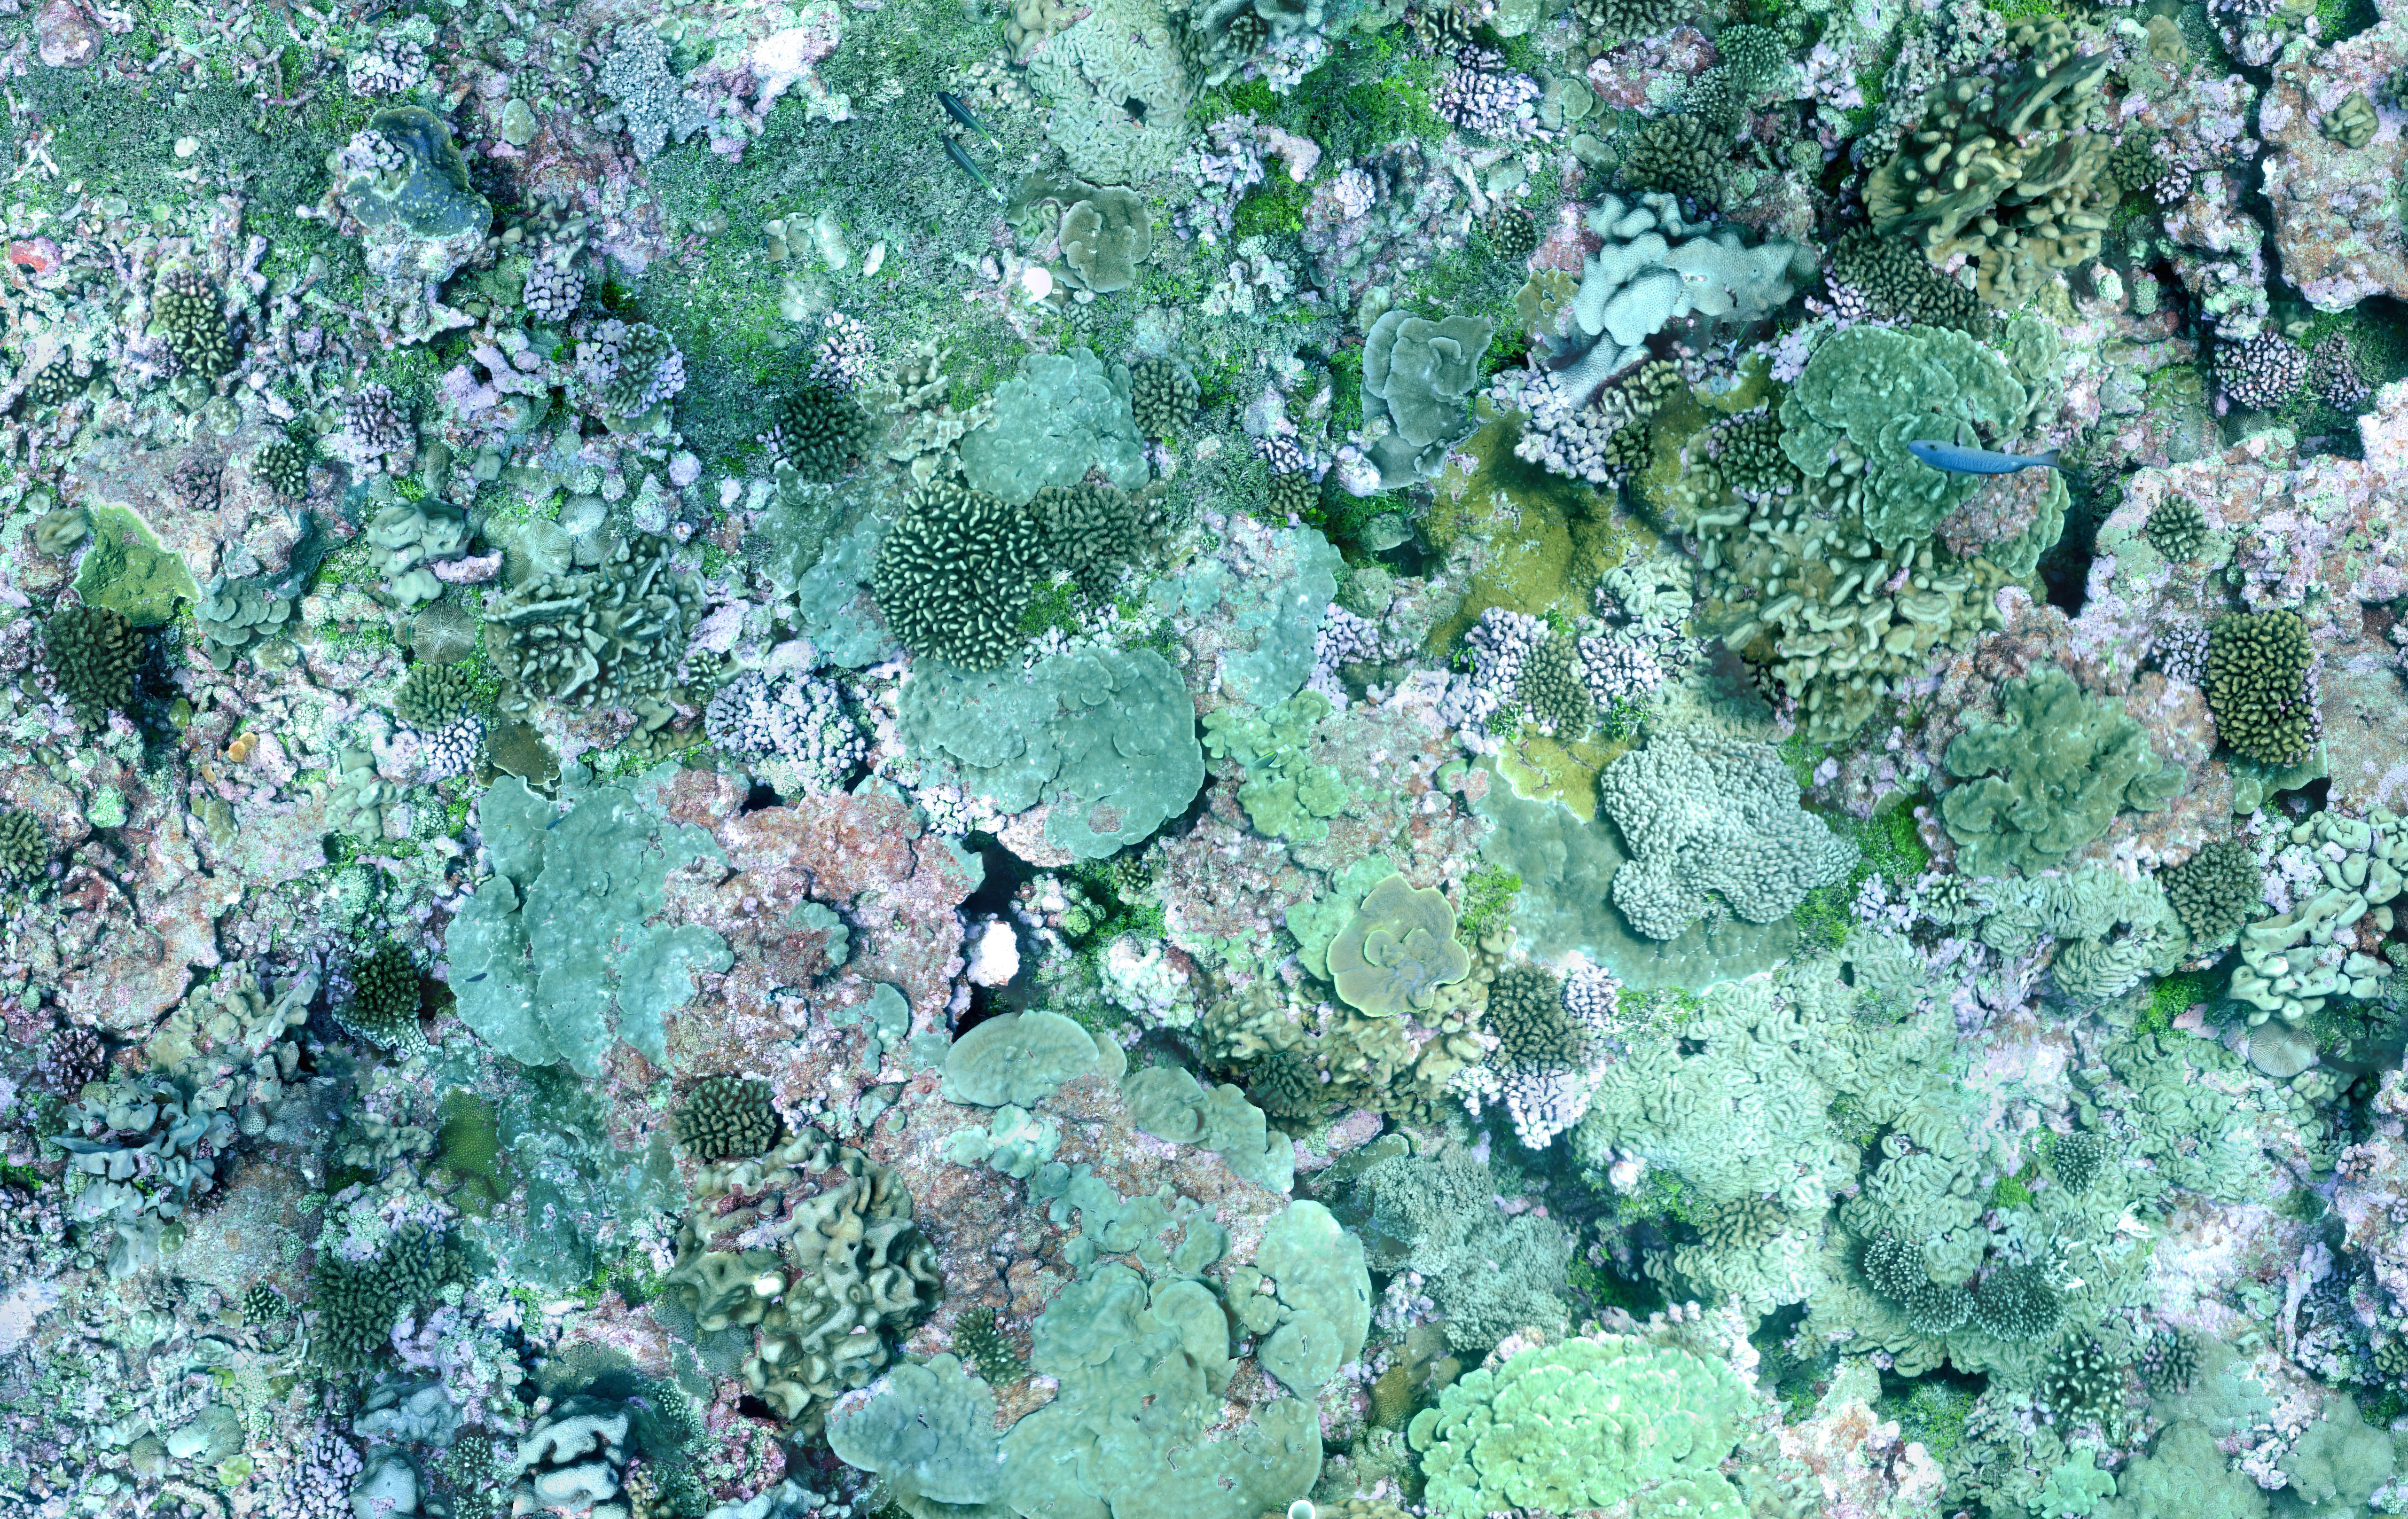
\includegraphics[width=5in]{coral/FR3_raw.jpg} 
   \caption{A portion of the raw photo-mosaic from Palmyra Island.}
   \label{coral_mosaic}
\end{figure}

\begin{figure}[htbp] %  figure placement: here, top, bottom, or page
   \centering
   \includegraphics[width=5in]{coral/FR3_class.jpg} 
   \caption{A portion of a classified photo-mosaic from Palmyra Island. Each color corresponds to a different coral or algae benthic species.}
   \label{classified_mosaic}
\end{figure}


Mosaics were collected in 2012 and again in 2013 at three islands within the Line Islands (Palmyra, Fanning, and Christmas). At each island, 20 meter by 20 meter zones were identified for monitoring and given a unique name for efficient data collection. Each island contains different human influence on coral reef habitat as the populations, water pollution, and sediment concentrations in the water vary between islands.  These varying degrees of human activity have caused correspondingly different levels of coral health \cite{line_islands_gradient} (Table \ref{coral_data}).  Manually classified mosaics for each of the islands studied here are shown in Figure \ref{coral_zones} where species have been coalesced into different morphological groupings.



\begin{table}[htbp]
\caption{Coral Zone Summary}
\begin{center}
\begin{tabular}{| l || c | c | c | c|}
  \hline       
  Zone & Location & Population & Coral Health & Study Sites\\
  \hline
  Palmyra & $5.8833^\circ$N, $162.0833^\circ$ W & 4 & Great & FR 3, 5, 7, 9 \\
  Fanning & $3.825^\circ$N, $162.349S^\circ$W & 2,500 & Good & FB 3, 4, 6, 9, 10, 11  \\
  Christmas &  $2.008^\circ$N, $157.489^\circ$W & 5,000 & Poor & KB4 \\
  \hline  
\end{tabular}
\end{center}
\label{coral_data}
\end{table}



\begin{figure}[htbp] %  figure placement: here, top, bottom, or page
   \centering
   \includegraphics[width=6in]{coral/coral_zones_all.pdf} 
   \caption{Manually classified photo-mosaics from Palmyra, Fanning, and Christmas islands. Each color corresponds to a different benthic morphological group. Image size is 1,500x1,500 pixels.}
   \label{coral_zones}
\end{figure}

















%


\newpage
%========================================================[DETERMINISTIC ANALYSIS]
\section{DETERMINISTIC ANALYSIS}


%=========================================================[BEACH ANALYSIS
\subsection{COASTAL ANALYSIS}

The non-linear forecasting technique is applied independently to the pre-nourishment and post-nourishment intertidal beach profiles (Figure \ref{beach}). The $R^2$ values are shown in Figure \ref{beach_contour_raw}.

\begin{figure}[htbp] %  figure placement: here, top, bottom, or page
   \centering
   \includegraphics[height=2in]{beach/beach_contour_raw.pdf} 
   \caption{Non-linear forecasting results for the pre-nourishment beach (left) and post-nourishment beach (right). The coefficient of determination, $R^2$, is plotted against near neighbors ($K$) and forecast distance.}
   \label{beach_contour_raw}
\end{figure}


The non-linear forecasting results show two very different trends. For the pre-nourishment beach, the $R^2$ values drop off more slowly than the post-nourishment beach for both forecast distance and near neighbors. One interpretation of the results for the pre-nourishment beach is that the high forecast skill over a relatively wide range of low $K$ and forecast distance indicates that the state space for the pre-nourishment beach is more populated than the post-nourishment beach.  Additionally, since forecast skill drops off more quickly for the post-nourishment beach, near neighbors in the state space do not evolve as similarly as the pre-nourishment beach. These trends seem to suggest that the nourishment episode abruptly moved the intertidal region away from its attractor and that it is slowly progressing back toward it's steady state and in doing so is dominated by internal system dynamics as opposed to responding to noisy forcing.

% Since the state space for the post-nourishment beach appears to be incomplete, the deterministic metric is not able to be calculated. Instead, to explore the day to day changes in the beach, the daily difference is calculated. The intent is to 



% \begin{figure}[htbp] %  figure placement: here, top, bottom, or page
%    \centering
%    \includegraphics[height=2.5in]{beach/beach_contour.pdf} 
%    \caption{Results of non-linear forecasting for the beach difference image. Color corresponds to the $R^2$ value.}
%    \label{beach_contour}
% \end{figure}

% \begin{figure}[htbp] %  figure placement: here, top, bottom, or page
%    \centering
%    \includegraphics[height=2.5in]{beach/beach_bar_plot.pdf} 
%    \caption{Deterministic metric calculated for the daily difference.}
%    \label{beach_bar}
% \end{figure}

%  Both images show a small peak at low number of near neighbors indicating that the system is deterministic and is not completely dominated by noise. The deterministic metric, however, indicates that the post-nourishment beach is slightly more deterministic than the pre-nourishment beach. This suggests that the large amount of fresh sand that was placed on the beach is more succeptible to internal dynamics. The sand is attempting to find a steady state and is more influenced by its shape than outside forcings such as waves.


%=========================================================[CORAL ANALYSIS]
\subsection{CORAL ANALYSIS}


The non-linear forecasting technique is applied to the coral images and the resulting contour plots of forecast skill are shown in Figure \ref{coral_contours}.

\begin{figure}[htbp] %  figure placement: here, top, bottom, or page
   \centering
   \includegraphics[width=5in]{coral/coral_contours.pdf} 
   \caption{Non-linear forecasting results for the coral zones. The percent correctly forecast, $P_c$, is plotted against near neighbors ($K$) and forecast distance.}
   \label{coral_contours}
\end{figure}

All zones display the same trend: highest $P_c$ values are obtained at low $K$ values and low forecast distances. This indicates that each zone is deterministic and that nearby regions in the reconstructed state space evolve similarly. Physically, this means that species on reefs influence the distribution of species around them. Assuming that all of zones are generated by the same dynamics (competition for benthic space between species on the coral reef) and that all of the state spaces are well populated, the deterministic metric can be compared across the various islands (Figure \ref{coral_bar}).
 
\begin{figure}[htbp] %  figure placement: here, top, bottom, or page
   \centering
   \includegraphics[width=5in]{coral/bar_plot_coral.pdf} 
   \caption{Deterministic metric, $D$, for the coral zones. The $x$-axis and color indicate location (green is Palmyra, yellow is Fanning, and red is Christmas).}
   \label{coral_bar}
\end{figure}

The metric shows a distinct trend with respect to each of the three islands with the highest values occurring at Palmyra. It appears as though the relatively pristine reefs of Palmyra have a more spatially deterministic structure, suggesting that non-linear internal spatial dynamics play a larger role in dictating benthic patterns at Palmyra than at the other islands in this study. The second grouping is four of the six Fanning Island zones. This indicates that there is still structure in the benthic patterning and that internal non-linear dynamics play a role in shaping the structure, but the relative influence of spatial noise is stronger than at Palmyra. The last grouping consists of three zones at Fanning and Christmas. These locations show  the least deterministic spatial structure according to the metric and these locations are in fact the most degraded of all the study zones. These results indicate that the non-linear forecasting technique coupled with the deterministic metric is able to distinguish relative reef health. This suggests that pollution and disturbance of the reef ecosystem destroys natural spatial relationships (non-linear internal dynamics) resulting in a benthic spatial structure that is more random.





\newpage


\section{CONCLUSION}

Collection of remote images of the nearshore region and photomosaics of the coral reef benthos has provided a series of spatiotemporal images of the upper shore-face and a series of spatial images along a gradient of coral reef degradation. Forecast skill from the novel application of both spatiotemporal nonlinear time series forecasting and the spatial analog suggest that the evolution of coastal and coral zones are governed by internal non-linear dynamics. Both forecast techniques elucidated the relative amount of stochasticity in the respective systems.

Although the metric was able to determine the relative amount of stochasticity within the systems, it does not provide an absolute measure of determinism across systems generated by different dynamics. For example, the absolute value of the deterministic metric was not able to capture the amount of determinism in the one-dimensional periodic equation when compared to the one-dimensional chaotic map. Moreover, the technique does not provide insight into the actual dynamics that generate a system. For the coral images, nothing is discovered concerning what spatial dynamics created the benthos other than the fact that the final configuration is deterministic.

The largest drawback of the technique is the large amount of data needed while the system is in it's steady state. Incomplete reconstructed state spaces result in forecast skill that mimics noise within the system even if the system is perfectly deterministic. Experimentation with small amounts of data for the one-dimensional chaotic map have shown suppressed $R^2$ values even for perfectly deterministic systems. Additionally, for high dimensional reconstructed state spaces, it is difficult to tell whether the system is in not in a steady state or the system is suffering from an incomplete attractor. This was apparent with the post-nourishment beach. The system most likely was not in a steady state, but it is also possible that the phase space for the post-nourishment beach is incomplete and more data is needed.

Nonetheless, the technique presented here was able to clearly distinguish the different system evolution for the pre-nourishment beach and post-nourishment as well as the different spatial configurations along the gradient of coral degradation. Likewise, the deterministic metric was able to succinctly illuminate the non-linear influence between near neighbors in the reconstructed state space between both the mathematical equations along a gradient of noise and natural systems (beach and coral). With significant human enterprise located in coastal regions around the world and the high economic benefit of coral reefs, there is a premium placed on the ability to understand coastline behavior and coral reef health. The results presented here suggest that image data coupled with nonlinear forecasting techniques can result in an insight into the evolution of the systems in time or space.

% **NEED TO LIST DRAWBACKS AND CAVEATS in a paragraph**
% 1) The metric is only good for comparing within system and does not provide an absolute measure of randomness vs determinism.

% 2) Embedding dim and lag values can not be set independently of the analysis.  Have attempted to set those values in a manner consistent with other authors.

% 3) The technique does not provide insight on what the dynamics actually are.

% 4) The technique requires a large amount of data and it requires data taken while the system is within it's attractor.  As shown for the beach, this can cause problems and it's often difficulty to identify whether a system is in the attractor.

% The methods used here do require choices for parameter values but some values, such as lags in the nonlinear forecasting technique, can be determined according to explicit tests that are not based on data fitting.











\newpage
\sectionx*{APPENDIX}
\addcontentsline{toc}{section}{APPENDIX}
\appendix

\section{IMPLEMENTATION OF THE NON-LINEAR FORECASTING TECHNIQUE}

The technique presented in this thesis was implemented in the Anaconda distribution of Python 2.7. Array manipulation was implemented in Numpy \cite{numpy}. Plotting was handled by Matplotlib \cite{matplotlib} and stylized by Seaborn \cite{seaborn}. The heart of the non-linear forecasting technique is the near neighbor algorithm from Sci-kit Learn \cite{scikit}. The work was completed in IPython Notebooks \cite{ipython}. The raw code for this project and accompanying IPython Notebooks can be found at nickc1.github.com.

The following subsections will go into more detail about the non-linear forecasting technique, but the general algorithm follows these steps:

\begin{enumerate}
\item Input one-dimensional time series or two-dimensional image.
\item Calculate the lag value which is the first minimum of the mutual information.
\item Split data into training set and testing set.
\item Embed each in an m-dimensional space.
\item Calculate the distance from all vectors in the test set to all vectors in the training set.
\item Average the evolution of the K closest vectors in the training set to make forecasts for the testing set.
\item Compare forecasts to actual evolution of the system.
\item Repeat steps 6 and 7 with K ranging from 1 to 25\% of the total size of the training set.
\item Repeat steps 4 through 8 to find the embedding dimension with highest forecast skill.
\item Calculate the Deterministic Metric.
\end{enumerate}
%=================================================

\subsection{LAG VALUE CALCULATION}
Before embedding a time series or an image, a lag value must be calculated. Lag values are given by the first minimum in the mutual information. A calculation of the mutual information for a time series, $X$, is implemented in python as:

\lstinputlisting[language=Python]{code_samples/mutual_information.py}

In this implementation, $X$ is the time series and $max\_lag$ is the maximum number of time steps that the time series is shifted. After shifting the time series and binning the time series values, sci-kit learn's mutual information implementation is calculated as,

$$MI(U,V) = \sum_{i=1}^R \sum_{j=1}^C P(i,j) log\frac{P(i,j)}{P(i)P'(j)}.$$

Here $P(i)$ is the probability of a random sample occurring in $U_i$ (the un-shifted time series) and $P'(j)$ is the probability of a random sample occurring in $V_j$ (the shifted time series). $P(i,j)$ is the probability of both $U_i$ and $V_j$ occurring in the same random sample. This function will output a series of mutual information values corresponding to the amount that the time series is shifted. For more information on lagged values for reconstructing state spaces refer to Reference \cite{mutual_info}.

For two-dimensional images, the mutual information along each row and each column is calculated and then summed together. This is implemented in python as,

\lstinputlisting[language=Python]{code_samples/spatial_mutual_info.py}

In this implementation $M$ is the input image, $max\_lag$ is the maximum amount of image shift, and $percent\_calc$ is the percent of rows and columns that are summed over to calculate the mutual information. The $percent\_calc$ is used to speed up the computation. Experimentation has shown that no accuracy is lost summing over a smaller amount of the rows or columns for the mutual information calculation. This function utilizes the one dimensional $mutual\_information$ function above.

%===========================================[Splitting into test and train set]
\subsection{TRAINING AND TESTING SETS}

When implementing the non-linear forecasting technique, the time series and images are split into a training set and a testing set. Usually, the training set consists of the first two-thirds of the data and the testing set is composed of the final one-third. By splitting the time series and images, forecasts for the test set using the training set can be compared to the actual values of the testing set. The accuracy of the forecasts can then be quantified. An implementation in python is given as,

\lstinputlisting[language=Python]{code_samples/2d_split.py}

This function is capable of handling both one dimensional and two dimensional inputs. The function utilizes the $try$, $except$ block to determine if the input is one dimensional or two dimensional.

%==========================================[Embedding]
\subsection{EMBEDDING}
The testing set and training sets are embedded independently in an m-dimensional space. The dimensionality, $m$, is iterated at a later step using a false near neighbors technique to determine the optimal embedding \cite{nonlinear_book}. An example of a single embedded vector of dimension 3 and a lag value of 2 for the first eight values of a time series, $T$ is given by the green squares in Figure \ref{1d_embedding}. 

\begin{figure}[htbp] %  figure placement: here, top, bottom, or page
   \centering
   \includegraphics[width=3in]{code/1d_reshape.pdf} 
   \caption{Embedding technique illustrating an embedding dimension of three with lag value of two. Green is the embedded time series values and red is the forecast y values.}
   \label{1d_embedding}
\end{figure}

The green squares are shifted by one to embed the next vector in the $m$-dimensional space. All of the embedded vectors are stored in a matrix, $X$. The red squares in Figure \ref{1d_embedding} represent the evolution vectors of the system. Likewise, the red squares are shifted over and the next evolution vector is obtained. These values are stored in a matrix $y$. The process is repeated for the embedded vectors and evolution vectors over the length of the time series. A generalization of this technique is given by:

\[
X=
\begin{bmatrix}
    T_{t} & T_{t+\tau} & T_{t+2\tau} & \dots  & T_{t+m\tau} \\
    T_{t+1} & T_{t+1 + \tau} & T_{t+1 + 2\tau} & \dots  & T_{t+1 +m\tau} \\
    \vdots & \vdots & \vdots & \ddots & \vdots \\
    T_{t+n} & T_{t+n+\tau} & T_{t+n + 2\tau} & \dots  & T_{t+ n+  m\tau}
\end{bmatrix}
\]

\[
Y=
\begin{bmatrix}
    T_{t+m\tau + 1} & T_{t+m\tau + 2}  & \dots  & T_{t+m\tau + p} \\
    T_{t+1 + m\tau + 1} & T_{t+1 + m\tau + 2}  & \dots  & T_{t+1 + m\tau + p} \\
    \vdots & \vdots & \vdots & \ddots & \vdots \\
    T_{t+n + m\tau + 1} & T_{t+n + \tau + 2}  & \dots  & T_{t+n +m\tau + p}
\end{bmatrix}
\]

Where $\tau$ is the lag value, $m$ is the embedding dimension, $p$ is the forecast distance, and $n$ is the length of $T$ minus the prediction distance. This implemented in python is given as,

\lstinputlisting[language=Python]{code_samples/lag_reshape.py}

The two-dimensional version of the embedding is similar to the time series version. An example embedding of a spatio-temporal image is given in Figure \ref{2d_embedding}. 

\begin{figure}[htbp] %  figure placement: here, top, bottom, or page
   \centering
   \includegraphics[width=3in]{code/2d_reshape.pdf} 
   \caption{Embedding technique illustrating an embedding dimension of six with lag value of two in both space and time. Green is the embedded spatio-temporal series values and red is the forecast y values.}
   \label{2d_embedding}
\end{figure}


The embedded vector (green) is six dimensional and has a spatial lag of 2 and a temporal lag of 2. The evolution vector is given in red. Both the embedded vector and the evolution vector are shifted over and the next embedded vector and evolution vector are calculated. The embedded vectors are stored in a matrix, $\vec X$, and the evolution vectors are stored in a matrix, $y$. Formally, $\vec X$ and $\vec Y$ can be defined as,

$$\vec X_{(t,s)}(x) = (x_{(t,s)}, x_{(t-\tau,s)}, \dots, x_{t-(m-1)\tau,s\pm \frac{n-1}{2}\sigma}),$$

$$\vec Y_{(t,s)}(x) = (x_{(t+1,s)}, x_{(t+2,s)}, \dots, x_{(t+p,s)}   ),$$

where $x$ is the spatio-temporal image, $s$ refers to the spatial component of the series, $\tau$ is the spatial lag, $\sigma$ is the spatial embedding dimension, and $p$ is the forecast distance. An implementation in python is given by:

\lstinputlisting[language=Python]{code_samples/ft_reshape.py}

This implementation allows for a certain percent of the space to be transformed into embedded vectors and evolution vectors. This is for computational efficiency in the calculation of distances. Furthermore, experimentation has shown that it is not necessary to test every single location. For most systems 25\% is effective. Additionally note that the lag values and embedding dimension are set up to be tuples. The first value is the lag or embedding dimension down the rows and the second value is across the columns. 


%=====================================================[KNN]
\subsection{K-NEAREST NEIGHBOR ALGORITHM}

At the heart of the non-linear forecasting technique is the K-Nearest Neighbors Algorithm \cite{nearest_neighbor}. The algorithm calculates the euclidean distances from each of the testing embedded vectors, $\vec X_{test}$ to each of the training embedded vectors, $\vec X_{train}$. The distance from the $i'th$ embedded train vector to the $j'th$ embedded test vector is,

$$ d_i( X_{train,i}, X_{test,j} ) = \sqrt{ (X_{train,i}-X_{test,j})^2}$$


The $y_{train}$ values of the closest $k$ vectors in the training set are averaged and a forecast, $y_p$, is made. This takes the form,

$$ y_{p} = \frac{ y_{train,1} + y_{train,2} + \dots  y_{train,k} } {k}. $$


The results of the forecast is then compared to the actual evolution vectors and the coefficient of determination, $R^2$ is calculated as,

$$R^2 = 1 - \frac{ \sum(y_i - f_i)^2 }  {\sum(y_i - \bar y )^2},$$

where $y_i$ is the $i^{th}$ prediction, $f_i$ is the true value, and $\bar y$ is the mean of the $y$ values. The near neighbor algorithm is implemented in python as,


\lstinputlisting[language=Python]{code_samples/nn_check.py}

This function utilizes sci-kit learn's $kneighbors$ function for efficient calculation of the distances from the testing set to the training set. It also has the ability to calculate weighted averages. For this paper, uniform weightings are used throughout.

In order to forecast discrete classes, the implementation is the same except the hamming distance is used to calculate the proximity of points and the mode of the $k$ nearest $y\_train$ class labels is the forecast where the mode is calculated as,

$$ Y_{p} = mode(y_{1}, y_{2}, \dots,  y_k). $$

This slightly different version is implemented in python as,

\lstinputlisting[language=Python]{code_samples/nnclassification.py}



Finally in order to evaluate the forecasts a metric is developed that calculates the percent correctly predicted. This is represented simply as,
$$ P = \frac{ N_c} {N_t}, $$
where $N_c$ is the number correctly predicted and $N_t$ is the total number of predictions. The algorithm is then iterated over a number of embedding dimensions $m$ to find the value of $m$ that gives the highest forecast skill. This is implemented in python as,


\lstinputlisting[language=Python]{code_samples/class_compare.py}

%===================================================== [Deterministic Metric]
\subsection{DETERMINISTIC METRIC}

The deterministic metric attempts to quantify the amount of determinism in a given time series or image. After finding the best embedding dimension, $m$, the algorithm is calculated as,

$$ D = \sum^n_{d=1} max(R^2_{d,\%K<12.5}) - min(R^2_{d,\%K\geq12.5}). $$

This function is implemented in python as,

\lstinputlisting[language=Python]{code_samples/deterministic_metric.py}



%====================================================[Example: One Dimensional]
\subsection{EXAMPLE: ONE-DIMENSIONAL}

Here the the $x$ values from the lorenz system are used to illustrate the workflow for the non-linear forecasting technique. The first step is to generate the time series and import the needed libraries. This is done as python as,

\lstinputlisting[language=Python]{code_samples/1d_example_lorenz_ts.py}

The required libraries are imported and Seaborn is used to style the plots. Scipy's integrate function is used to integrate the lorenz equations. The resulting plot is shown in Figure \ref{create_series}.

\begin{figure}[htbp] %  figure placement: here, top, bottom, or page
   \centering
   \includegraphics[width=3in]{code/lorenz_ts.pdf} 
   \caption{$X$ values from the lorenz equations.}
   \label{create_series}
\end{figure}


The next step is to calculate a lag value for the system. This is done by finding the first minimum of the mutual information between a shifted time series and an unshifted one. The results of the code are shown in Figure \ref{code_mutual_info}.

\lstinputlisting[language=Python]{code_samples/1d_example_mutual_info.py}

\begin{figure}[htbp] %  figure placement: here, top, bottom, or page
   \centering
   \includegraphics[width=3in]{code/lorenz_mutual_info.pdf} 
   \caption{Mutual information between the shifted $X$ values and unshifted $X$ values from the lorenz equations.}
   \label{code_mutual_info}
\end{figure}

Now we can split our time series into a testing set and a training set. This is done in python as,

\lstinputlisting[language=Python]{code_samples/1d_example_split.py}


The next step is to iterate over the embedding dimension $m$ to find the embedding that provides the maximum forecast skill. This takes three functions: $nnEfficient$, $score$, and $em\_check$. $em\_check$ iterates through $m$ to find the ideal embedding, while $nnEfficient$ finds the near neighbors in the reconstructed state space. $score$ quantifies the forecast skill. The results are shown in Figure \ref{best_embedding}

\lstinputlisting[language=Python]{code_samples/1d_example_find_embedding.py}

\begin{figure}[htbp] %  figure placement: here, top, bottom, or page
   \centering
   \includegraphics[width=3in]{code/lorenz_best_em.pdf} 
   \caption{Coefficient of determination $R^2$ versus embedding dimension, $m$.}
   \label{best_embedding}
\end{figure}

According to the ideal embedding for the time series is two. This is then used to embed our data. We can visualize the embedding through the code below that produces Figure \ref{code_embedding}.


\lstinputlisting[language=Python]{code_samples/1d_example_embedded_lorenz.py}

\begin{figure}[htbp] %  figure placement: here, top, bottom, or page
   \centering
   \includegraphics[width=3in]{code/lorenz_embedded.pdf} 
   \caption{Two-dimensional embedding of the lorenz $X$ values.}
   \label{code_embedding}
\end{figure}



Finally we can run $nnEfficient$ and produce a contour plot of the results in order to visualize the trends in forecast skill with respect to the number of neighbors used. The code below produces Figure \ref{code_contour}


\lstinputlisting[language=Python]{code_samples/1d_example_final_step.py}

\begin{figure}[htbp] %  figure placement: here, top, bottom, or page
   \centering
   \includegraphics[width=3in]{code/lorenz_contour.pdf} 
   \caption{Coefficient of determination $R^2$ versus embedding dimension, $m$.}
   \label{code_contour}
\end{figure}









% $$X = y$$

% where, 
% \[
% X=
% \begin{bmatrix}
%     x_{11} & x_{12} & x_{13} & \dots  & x_{1n} \\
%     x_{21} & x_{22} & x_{23} & \dots  & x_{2n} \\
%     \vdots & \vdots & \vdots & \ddots & \vdots \\
%     x_{d1} & x_{d2} & x_{d3} & \dots  & x_{dn}
% \end{bmatrix}
% \]

% \[
% y=
% \begin{bmatrix}
%     y_{11} & y_{12} & y_{13} & \dots  & y_{1n} \\
%     y_{21} & y_{22} & y_{23} & \dots  & y_{2n} \\
%     \vdots & \vdots & \vdots & \ddots & \vdots \\
%     y_{d1} & y_{d2} & y_{d3} & \dots  & y_{dn}
% \end{bmatrix}
% \]

% $X$ is referred to as the features (the variables that are used to predict $y$) and $y$ is referred to as the target variables. Each sample, $d$, has dimensionality $n$. This is to say, $(x_{d1}, x_{d2}, x_{d3}, \dots, x_{dn})$ is used to predict $(y_{d1}, y_{d2}, y_{d3}, \dots, y_{dn})$.




% In order to make predictions about a single sample in the testing set, the euclidean distance from the feature vectors in the testing set to the feature vectors in the training set are calculated as:

% $$ d( (x_{rd1},x_{rd2}, \dots, x_{rdn}) , (x_{td1},x_{td2}, \dots, x_{tdn}) ) =$$
% $$ \sqrt{ (x_{rd1}-x_{td1})^2 + (x_{rd2}-x_{td2})^2 + \dots + (x_{rdn}-x_{tdn})^2  }$$

% The $y_r$ values of the closest $k$ vectors in the training set are averaged together to make a prediction, $Y_p$ about the testing set. This takes the form,

% $$ Y_{p} = \frac{ y_{1} + y_{2} + \dots  y_k } {k}. $$

% If the prediction is a discrete class label, then the mode is taken. This takes the form,

% $$ Y_{p} = mode(y_{1}, y_{2}, \dots,  y_k) $$

% After predicting all of the samples appropriately, the next step is to make some measurement about the accuracy of the predictions. For regression problems, the coefficient of determination is calculated as,

% $$R^2 = 1 - \frac{ \sum(y_i - f_i)^2 }  {\sum(y_i - \bar y )^2}$$

% Where $y_i$ is the $i$ prediction, $f_i$ is the true value, and $\bar y$ is the mean of the $y$ values. 

% For classification problems, the percent correctly predicted is calculated as, 

% $$ P = \frac{ N_c} {N_t}, $$

% where $N_c$ is the number correctly predicted and $N_t$ is the total number of predictions.


% %===================================================[One Dimensional Regression]
% \subsection{One Dimensional Regression}

% To apply the near neighbor algorithm to a time series, first the time series must be embedded in order to apply the algorithm. Given a time series $T$, it is reshaped to produce a set of feature vectors $X$ and a set of target vectors $y$ and take the form of,

% \[
% X=
% \begin{bmatrix}
%     T_{t} & T_{t+\tau} & T_{t+2\tau} & \dots  & T_{t+m\tau} \\
%     T_{t+1} & T_{t+1 + \tau} & T_{t+1 + 2\tau} & \dots  & T_{t+1 +m\tau} \\
%     \vdots & \vdots & \vdots & \ddots & \vdots \\
%     T_{t+n} & T_{t+n+\tau} & T_{t+n + 2\tau} & \dots  & T_{t+ n+  m\tau}
% \end{bmatrix}
% \]

% \[
% Y=
% \begin{bmatrix}
%     T_{t+m\tau + 1} & T_{t+m\tau + 2}  & \dots  & T_{t+m\tau + p} \\
%     T_{t+1 + m\tau + 1} & T_{t+1 + m\tau + 2}  & \dots  & T_{t+1 + m\tau + p} \\
%     \vdots & \vdots & \vdots & \ddots & \vdots \\
%     T_{t+n + m\tau + 1} & T_{t+n + \tau + 2}  & \dots  & T_{t+n +m\tau + p}
% \end{bmatrix}
% \]

% where $\tau$ is the lag value, $m$ is the embedding dimension, $p$ is the forecast distance, and $n$ is the length of $T$ minus the prediction distance. 

% After reshaping the time series into feature vectors, $X$, and a target vectors, $y$, the vectors must be split into a traing set and a testing set. A python implementation is given by,

% \newpage
% \lstinputlisting[language=Python]{code_samples/train_test_split.py}

% Next, the reshaped training set and testing set can be fed into a near neighbor algorithm. Here, an implementation in Sci-kit Learn is used.

% \newpage
% \lstinputlisting[language=Python]{code_samples/nn_check.py}

% All the pieces have been coded, now everything is given one wrapper function so that a time series can be given and out pops the analysis over a range of near neighbors.


% \newpage
% \lstinputlisting[language=Python]{code_samples/train_predict.py}




% %====================================================[Two-Dimensional Regression]
% \subsection{Two-Dimensional Regression}

% Now to extend the algorithm to two dimensions, all that needs to be done is to alter the reshaping technique. Other than that, everything is the same. Feature vectors in the spatial sense are represented as: 

% $$y_{(t,s)}(x) = (x_{t,s)}, x_{(t-\tau,s)}, \dots, x_{t-(m-1)\tau,s\pm \frac{n-1}{2}\sigma})$$

% \begin{figure}[htbp] %  figure placement: here, top, bottom, or page
%    \centering
%    \includegraphics[width=3in]{code/2d_reshape.pdf} 
%    \caption{Embedding technique illustrating an embedding dimension of six with lag value of two in both space and time. Green is the embedded spatio-temporal series values and red is the forecast y values.}
%    \label{raw_data}
% \end{figure}



% An implementation in python is given by:

% \newpage
% \lstinputlisting[language=Python]{code_samples/ft_reshape.py}

% \newpage
% \lstinputlisting[language=Python]{code_samples/spatial_mutual_info.py}

% Additionally, splitting the space into a training set and a test set before makes the process easier. The two dimensional splitting function is represented as:

% \newpage
% \lstinputlisting[language=Python]{code_samples/2d_split.py}

% The whole two-dimensional regression technique is then wrapped into one function as:

% \newpage
% \lstinputlisting[language=Python]{code_samples/train_predict_2d.py}


% %=====================================================[Two-Dimensional Classification]
% \subsection{TWO-DIMENSIONAL CLASSIFICATION}


% The two dimensional classification is the same as the two-dimensional regression except for the classification algorithm which is represented as:

% \newpage
% \lstinputlisting[language=Python]{code_samples/nnclassification.py}

% Also the scoring function


% \newpage
% \lstinputlisting[language=Python]{code_samples/class_compare.py}


% \newpage
% \lstinputlisting[language=Python]{code_samples/full_usage.py}






% % \[x_{pred}(X_{c})=
% % \begin{cases} 
% %     1 &  \text{if } max(X_1,X_2,\dots,X_c) = X_1 \\
% %     2 &  \text{if } max(X_1,X_2,\dots,X_c) = X_2 \\
% %     \vdots \\
% %     c &  \text{if } max(X_1,X_2,\dots,X_c) = X_c
% %  \end{cases}
% % \]



% % \[F(x_t)=
% % \begin{cases} 
% %     1 &  \text{if } x_{t} = x_{pred} \\
% %     0 &  \text{if } x_{t} \neq x_{pred}
% %  \end{cases}
% % \]


% \clearpage
% %=====================================================[knn-classification]
% \subsection{Classification Example}
% The  In this section we will observe it classifying samples into one of five possible classes. Below, some test data was generated and can be seen in Figure \ref{raw_data}. This data has two features $(x_{d1},x_{d2})$, contains 100 samples, and has one target variable, $y_{d1}$, that can be one of five classes. 

% The first thing to do with this test data is the split it into a training set and a test set. We then calculate the distance between each test sample and each of the training samples. For each of the test samples, a weighted mode of the $k$ closest samples in the test set is taken. It turns out that for different numbers of $k$, we obtain different numbers of correctly classified points. This can be seen in Figure \ref{changing_k_plot}.

% One way to visualize why the percent of correctly identified points change is by this is by drawing a decision boundary as seen in Figure \ref{changing_k}. Each color in the plot corresponds to any point in that region being classified as that class. We can see that most of the points have been classified correctly, but as we increase $k$ the regions change shape. While for this example, it is slightly trivial, we will see the importance of near neighbor behavior in later examples.


% \begin{figure}[htbp] %  figure placement: here, top, bottom, or page
%    \centering
%    \includegraphics[height=3in]{code/raw_data.pdf} 
%    \caption{Example data.}
%    \label{raw_data}
% \end{figure}

% \begin{figure}[htbp] %  figure placement: here, top, bottom, or page
%    \centering
%    \includegraphics[height=3in]{code/decision_boundary.pdf} 
%    \caption{Example data with a boundary drawn in. K=5.}
%    \label{decision_boundary}
% \end{figure}


% \begin{figure}[htbp] %  figure placement: here, top, bottom, or page
%    \centering
%    \includegraphics[height=3in]{code/changing_k.pdf} 
%    \caption{Changing decision boundary based on the number of near neighbors.}
%    \label{changing_k}
% \end{figure}

% \begin{figure}[htbp] %  figure placement: here, top, bottom, or page
%    \centering
%    \includegraphics[height=3in]{code/changing_k_plot.pdf} 
%    \caption{Changing percent correct based on the number of near neighbors.}
%    \label{changing_k_plot}
% \end{figure}


% \clearpage
% %=====================================================[knn-regression]
% \subsection{Regression}
% In this section, we will explore the $k$-nearest neighbor algorithm for regression. Following the same logic above, we find the points that are closest to the point in question and calculate the mean. Likewise, it is best illustrated with an example. An example of using KNN for regression can be seen in Figure \ref{data_regression}. For this example we have generated some test points using a sine wave with a little bit of noise added on top. We will then take two-thirds of this data and use it as our training set. We will then make predictions based on the closest number of points. Again, we will be using the euclidean distance.

% After running the algorithm for different number of near neighbors, we see behavior like that shown in \ref{multiple_subplots_regression}. As we can see from the plots, as you increase the number of near neighbors, the behavior of the predictions becomes more subtle and is not a badly overfit.

% As is seen in Figure \ref{changing_k_regression}, the amount of near neighbors has about a $0.15$ difference in the $R^2$ value where $R^2$ is calculated as,



% In this expression, $y_i$ is the actual value, $f_i$ is the predicted value, and $\bar y$ is the mean of the actual values. Interestingly, we see the behavior that as we increase the number of near neighbors, our predictions get better and better. We will see this behavior again in the later sections.

% \begin{figure}[htbp] %  figure placement: here, top, bottom, or page
%    \centering
%    \includegraphics[height=3in]{code/data_regression.pdf} 
%    \caption{Data was generated using a sine wave with a little bit of noise added.}
%    \label{data_regression}
% \end{figure}


% \begin{figure}[htbp] %  figure placement: here, top, bottom, or page
%    \centering
%    \includegraphics[height=3in]{code/multiple_k_subplots.pdf} 
%    \caption{Results of predicting on one third of the data. Title is the amount of near neighbors used.}
%    \label{multiple_subplots_regression}
% \end{figure}


% \begin{figure}[htbp] %  figure placement: here, top, bottom, or page
%    \centering
%    \includegraphics[height=3in]{code/changing_k_regression} 
%    \caption{$R^2$ for prediction on one third of the data.}
%    \label{changing_k_regression}
% \end{figure}

% \subsection{Summary}
% So we have seen two ways that the K-nearest neighbor algorithm works--one classification example and one regression example. In these two examples, we only had one or two features with a single target. This algorithm will use the same fundamental principles, but b





%\input{./chapters/beach}
%\input{./chapters/coral}



%\input chap2
\newpage
%\sectionx*{REFERENCES}
\addcontentsline{toc}{section}{REFERENCES}
\bibliographystyle{plain}
\bibliography{citations.bib}
\clearpage

%\input biblio
%\input appendix
%
% Biographical Sketch (Optional for Graduate School)
%
%\newpage
%\begin{singlespace}
%\section*{BIOGRAPHICAL SKETCH}
%Here is the section where you can let the reader know something
%about your educational background and any other pertinent
%professional information that you would like the reader to know.
%\end{singlespace}
\end{document}




